% Provenance (never printed): see sources/outline_sources.md (Year 2: climate archives and proxies;
% foraminiferal and ice isotopes; Mg/Ca; pollen; speleothems; tree rings; dating the archives).
% Calibrations after Miller et al. (2020), Groeneveld et al. (2019) and Morley et al. (2024); ice
% cores after White (Geochemistry, ch. 9), Werner et al. (2018) and the EPICA Dome C file of Jouzel
% et al. (2007); age model after Svensson et al. (2008); deep-water context after Wharton et al.
% (2026); figures from figdata/bachelor-2/proxies.py (data/derived lr04, edc-temperature,
% co2-icecore); values of the exercises and problem computed in the Book 4 scratch calculator
% calc/ch24.py.
\chapter{الأرشيفات والمؤشّرات المناخية البديلة}\label{ch:b2:climate-proxies}

في بحث نُشر عام 1955 قاس كيميائي جيولوجي شابّ نظائر الأكسجين في الأصداف الدقيقة
للمنخربات المنتقاة من عيّنات لبّية من قاع المحيط، فوجد فيها خمس عشرة دورة جليدية--بين جليدية على مدى
\num{600000} سنة الأخيرة. وقد قرأها في معظمها على أنها درجة حرارة: فلم ينسب إلا نحو الخمس من
التأرجحات إلى الجليد المختزن على اليابسة. وبعد ثماني عشرة سنة، خلص شاكلتون وأوبدايك إلى
العكس: فالأثر الرئيسي كان اختزان الماء الخفيف نظائريًّا في الأغطية
الجليدية. الأصداف نفسها، والأرقام نفسها، وقراءتان. فصدفة الكالسيت تسجّل
درجة حرارة الماء الذي نمت فيه وتركيب ذلك الماء، وتركيب
ماء البحر يتوقّف على مقدار الجليد على اليابسة. يتناول هذا الفصل مثل هذه السجلّات،
والأرشيفات التي تحفظها، والمؤشّرات البديلة التي تُقرأ منها، وكيف تُعايَر مقابل موازين الحرارة
وكيف تُؤرَّخ، وفنّ الفصل بين إشارتين تحملهما صدفة واحدة.
% ledger: white13c9:paleo-history

\begin{recall}
\textbf{من مجلّدات المدرسة}: \omterm{def:b2:climate-proxies:proxy}{الأرشيف المناخي} \omterm{def:b2:climate-proxies:proxy}{والمؤشّر البديل}، والعيّنة الجليدية، والفترة الجليدية
والفترة بين الجليدية، والذروة الجليدية الأخيرة (قبل نحو \num{23000} إلى \num{19000} سنة)، وتحليل
حبوب اللقاح. \textbf{من مجلد السنة الأولى}: التأريخ الإشعاعي، وعمر الكربون المشعّ
ومنحنى معايرته؛ والرسوب الكلسي الناعم، المكوّن من الكوكوليثات وأصداف المنخربات.
\textbf{من \cref{ch:b2:isotope-geochemistry}}: المعياران النظائريان المرجعيان \omterm{def:b2:isotope-geochemistry:standards}{VSMOW} \omterm{def:b2:isotope-geochemistry:standards}{وVPDB}
(\cref{def:b2:isotope-geochemistry:standards}) وخطّ الماء الجوّي، $\delta\mathrm{D}
\approx 8\,\delta^{18}\mathrm{O} + 10$ (\cref{prop:b2:isotope-geochemistry:mwl}). \textbf{من
كتب الكيمياء}: القيمة $\delta$ ومعامل التجزئة. \textbf{من كتب
الرياضيات}: مستقيم المربّعات الصغرى.
\end{recall}
% ledger: ipcc:lgm-cooling, kc98:mwl, kc98:standards

\section{الأرشيفات والمؤشّرات البديلة}\label{sec:b2:climate-proxies:archives}

لم تقس الأجهزة المناخ إلا منذ وقت قريب. وكلّ ما سبق ذلك يُقرأ من موادّ
نمت أو ترسّبت طبقة فوق طبقة بينما كان المناخ يؤثّر فيها: ثلج يتحوّل إلى جليد على
الأغطية الجليدية القطبية، وأصداف تتساقط على قاع المحيط، وحلقات الأشجار، والمرجان، ورواسب
الكهوف، وطين البحيرات. وقد سمّتها مجلّدات المدرسة أرشيفات وسمّت الكمّيات المقيسة
فيها مؤشّرات بديلة؛ ونحتاج الآن إلى كلمات أدقّ.

\begin{definition}[الأرشيف المناخي؛ المؤشّر البديل]\label{def:b2:climate-proxies:proxy}
\emph{الأرشيف المناخي}\index{الأرشيف المناخي} مادة طبيعية تتراكم
تدريجيًّا، طبقة فوق طبقة أو حلقة فوق حلقة، وتحفظ خصائص فيزيائية أو كيميائية أو حيوية
للبيئة التي تكوّن فيها كلّ جزء منها. و\emph{المؤشّر
البديل}\index{المؤشّر البديل} كمّية تُقاس في أرشيف وتتوقّف على متغيّر مناخي،
كدرجة حرارة أو كمّية مطر أو حجم جليد، عبر علاقة يمكن
معايرتها، فتقوم مقام قياس لذلك المتغيّر لم يُجرَ قطّ.
\end{definition}
% ledger: ncei:proxy, ncei:paleocean

ثلاث خصائص تحدّد ما يستطيع الأرشيف أن يخبر به: دقّته الزمنية (المدّة الزمنية التي تغطّيها
عيّنة واحدة)، ومداه (إلى أيّ زمن يعود)، وطريقة تأريخه. فالأرشيف ذو الطبقات السنوية يمكن
قراءته سنة بسنة وتأريخه بالعدّ؛ أمّا الأرشيفات الأخرى فتحتاج إلى أعمار إشعاعية أو إلى مقارنة بسجلّ
مؤرَّخ. ويقارن الجدول أدناه بين أرشيفات هذا الفصل.

\begin{center}
\small
\begin{tabular}{>{\raggedright\arraybackslash}p{0.17\linewidth}>{\raggedright\arraybackslash}p{0.27\linewidth}>{\raggedright\arraybackslash}p{0.21\linewidth}>{\raggedright\arraybackslash}p{0.24\linewidth}}
\hline
الأرشيف & المؤشّرات البديلة في هذا الفصل & طبقات سنوية & التأريخ \\
\hline
الرسوبيات البحرية العميقة & \mbox{\textdir TLT $\delta^{18}$O} وMg/Ca في المنخربات & لا & الكربون المشعّ، والمقارنة بسجلّات
مؤرَّخة \\
الجليد القطبي & \mbox{\textdir TLT $\delta$D} و\mbox{\textdir TLT $\delta^{18}$O} في الجليد، والهواء في الفقاعات & في الجزء العلوي من العيّنات
الطويلة & عدّ الطبقات، وطبقات بركانية مؤرَّخة \\
حلقات الأشجار & عرض الحلقة، وكثافة الخشب، والنظائر & نعم & عدّ الحلقات \omterm{def:b2:climate-proxies:dendro}{والتأريخ المتقاطع} \\
\omterm{def:b2:climate-proxies:archives}{الرواسب الكهفية} & \mbox{\textdir TLT $\delta^{18}$O} & في بعضها & التأريخ الإشعاعي \\
رسوبيات البحيرات & الفارفات، وحبوب اللقاح & حيث توجد الفارفات & عدّ الفارفات \\
\hline
\end{tabular}
\end{center}
% ledger: ncei:proxy, ncei:paleocean, ncei:tree-ring, ncei:speleothem, mccarthy23:varves, svensson08:gicc05, noaa:gisp2-layers, bebchuk26:crossdating

\omterm{def:b2:climate-proxies:proxy}{المؤشّر البديل} ليس أبدًا مقياسًا خالصًا لمتغيّر واحد. فعرض حلقة الشجرة يتوقّف على دفء
الصيف وعلى المطر؛ و\mbox{\textdir TLT $\delta^{18}$O} في الصدفة على درجة حرارة الماء وعلى
تركيبه النظائري. وعمل عالم المناخ القديم هو إيجاد مؤشّر بديل يكون اعتماده
على المتغيّر المطلوب قويًّا ومعروفًا، وقياس المؤثّرات الأخرى قياسًا مستقلًّا،
وتأريخ العيّنة.

\section{نظائر الأكسجين في الأصداف الكربوناتية}\label{sec:b2:climate-proxies:oxygen}

المنخربات طلائعيات وحيدة الخلية، يبني كثير منها صدفة من الكالسيت؛ فالأنواع العوالق
تطفو في المياه السطحية، والأنواع القاعية تعيش على رسوبيات قاع البحر أو
داخلها. وتتراكم أصدافها في الرسوب الكلسي الناعم الذي عرضه مجلد السنة الأولى، ويمكن قياس
\mbox{\textdir TLT $\delta^{18}$O} في كالسيتها على بضع أصداف تُنتقى من كلّ سنتيمتر من
العيّنة اللبّية.
% ledger: ucmp:forams, ncei:paleocean

\begin{history}[قراءتان لسجلّ واحد]
حسب يوري عام 1947 كيف تتوقّف تجزئة الأكسجين بين الكالسيت والماء على
درجة الحرارة، واقترح أن الكربونات قد تسجّل درجة الحرارة التي تكوّنت عندها. ثم قاس تشيزاري
إميلياني، تلميذه آنذاك، \mbox{\textdir TLT $\delta^{18}$O} في منخربات من عيّنات لبّية مكبسية من
محيطات العالم ونشر عام 1955 سجلًّا فيه 15 دورة جليدية--بين جليدية على مدى
\num{600000} سنة، ناسبًا نحو \qty{20}{\percent} من التغيّر إلى حجم الجليد.
وفي عام 1973 خلص شاكلتون وأوبدايك إلى أن اختزان الماء الخفيف نظائريًّا في
الأغطية الجليدية كان الأثر الرئيسي. أمّا الآثار الحيوية، أي انحرافات نوع ما عن التوازن،
وتبادل الأكسجين مع ماء المسام بعد الدفن، فليست عادةً ذات أهمية كبيرة في
أصداف ملايين السنين القليلة الأخيرة؛ أمّا التركيب النظائري للماء فمهمّ.
\end{history}
% ledger: white13c9:paleo-history

\subsection*{درجة الحرارة}

الكالسيت الذي ينمو في توازن مع الماء أغنى من الماء بالنظير \textsuperscript{18}O،
وكلّما كان الماء أبرد كان الإغناء أكبر، كما بيّن حساب يوري. وتربط عدّة
معايرات تجريبية
درجة الحرارة بالفرق بين \mbox{\textdir TLT $\delta^{18}$O} في الكالسيت، على مقياس \omterm{def:b2:isotope-geochemistry:standards}{VPDB}،
ونظيره في الماء، على مقياس \omterm{def:b2:isotope-geochemistry:standards}{VSMOW}. ففي البحر العميق تُستعمل صيغة مبسّطة للأصداف
القاعية.

\begin{proposition}[معايرة للمنخربات القاعية]\label{prop:b2:climate-proxies:benthic}
للمنخربات القاعية عند درجات حرارة البحر العميق (دون نحو \qty{13}{\celsius})،
\[
  T = 16.1 - 4.76\,\bigl[\delta^{18}\mathrm{O}_{\mathrm{b}} - (\delta^{18}\mathrm{O}_{\mathrm{sw}} -
  0.27)\bigr],
\]
حيث $T$ بوحدة \unit{\celsius}، و$\delta^{18}\mathrm{O}_{\mathrm{b}}$ قيمة الصدفة (بالجزء في الألف،
\omterm{def:b2:isotope-geochemistry:standards}{VPDB}) و$\delta^{18}\mathrm{O}_{\mathrm{sw}}$ قيمة ماء البحر (بالجزء في الألف، \omterm{def:b2:isotope-geochemistry:standards}{VSMOW})؛ والحدّ
0.27 يحوّل الماء إلى مقياس الكالسيت. والتبرّد بمقدار \qty{1}{\celsius} مع ثبات
تركيب الماء يرفع $\delta^{18}\mathrm{O}_{\mathrm{b}}$ بمقدار $1/4.76 = 0.21$ بالجزء في الألف.
\end{proposition}
\admitted
% ledger: miller20:paleotemp, groeneveld19:anand

المعادلة الأكمل التي بُسّطت منها تتضمّن حدًّا تربيعيًّا صغيرًا،
$T = 16.1 - 4.64x + 0.09x^2$ حيث $x$ الفرق بين قيمتي $\delta$؛ وللأصداف العوالق
معايراتها الخاصة، من الشكل نفسه، مثل $T = 14.9 - 4.8\,[\delta^{18}\mathrm{O} -
(\delta^{18}\mathrm{O}_{\mathrm{sw}} - 0.27)]$. وتشترك كلّها في صعوبة واحدة: فالصدفة تعطي
عددًا واحدًا، $\delta^{18}\mathrm{O}_{\mathrm{b}}$، والمعادلة فيها مجهولان، $T$
و$\delta^{18}\mathrm{O}_{\mathrm{sw}}$. ويلزم مؤشّر بديل ثانٍ مستقلّ للفصل بينهما.
% ledger: miller20:paleotemp, groeneveld19:anand

\subsection*{أثر حجم الجليد}

الماء المتبخّر من البحر يحمل من النظير \textsuperscript{18}O أقلّ ممّا يحمله البحر؛ ومع انتقال البخار
نحو القطب وسقوطه مطرًا أو ثلجًا، يزداد فقره، والثلج الذي يبني الأغطية
الجليدية من أخفّ مياه الكوكب: فجليد غرينلاند قيمة \mbox{\textdir TLT $\delta^{18}$O} فيه من $-30$ إلى $-35$
بالجزء في الألف، وجليد القارة القطبية الجنوبية حتى $-50$. وحين تنمو الأغطية الجليدية، يُحتجز النظير الخفيف على اليابسة
ويصبح المحيط الباقي أثقل.
% ledger: nasaeo:o18, white:d18o

\begin{definition}[أثر حجم الجليد]\label{def:b2:climate-proxies:ice-volume}
\emph{أثر حجم الجليد}\index{أثر حجم الجليد} هو تغيّر التركيب النظائري للأكسجين
في المحيط كلّه بسبب نموّ الأغطية الجليدية القارّية أو تلاشيها، وهي
تختزن ماءً فقيرًا بالنظير \textsuperscript{18}O؛ فهو يزيح \mbox{\textdir TLT $\delta^{18}$O} في كلّ كربونات
تكوّنت في البحر بالمقدار نفسه، أيًّا كانت درجة الحرارة.
\end{definition}
% ledger: nasaeo:o18, white13c9:ice-volume, miller20:paleotemp

\begin{omfigure}
\centering
\begin{tikzpicture}[font=\scriptsize, >=Stealth]
\foreach \col/\title in {0/{أ\enspace اليوم}, 7.0/{ب\enspace ذروة جليدية}} {
  \begin{scope}[shift={(\col,0)}]
  \node[anchor=south west] at (0,3.3) {\textbf{\title}};
  \fill[brown!30] (3.6,0) -- (6.4,0) -- (6.4,1.6) -- (3.6,1.2) -- cycle;
  \end{scope}
}
% today: full ocean, small ice sheet
\fill[ocBlue!25] (0,0) rectangle (3.6,1.2);
\node[align=center] at (1.75,0.55) {محيط\\$\delta^{18}\mathrm{O} = 0$};
\fill[white, draw=black!50] (5.2,1.43) .. controls (5.6,1.95) and (6.2,1.95) .. (6.4,1.6) -- cycle;
\node at (5.0,0.65) {\foreignlanguage{arabic}{جليد، $-40$}};
\draw[black!50] (5.0,0.85) -- (5.7,1.55);
\draw[->, thick, ocBlue] (1.6,1.35) .. controls (2.4,2.9) and (4.6,2.9) .. (5.6,2.05);
\node at (3.4,3.0) {بخار خفيف};
% glacial: lower sea, big ice sheet
\begin{scope}[shift={(7.0,0)}]
\fill[ocBlue!35] (0,0) rectangle (3.6,0.85);
\draw[densely dashed] (0,1.2) -- (3.6,1.2);
\node[anchor=south west, align=left] at (0.05,1.2) {مستوى البحر\\اليوم};
\draw[<->] (3.35,0.85) -- (3.35,1.2);
\node[anchor=east] at (3.3,1.02) {\qty{130}{m}};
\node[align=center] at (1.6,0.42) {\foreignlanguage{arabic}{محيط، $\delta^{18}\mathrm{O} = +1.46$}};
\fill[white, draw=black!50] (3.6,1.2) .. controls (4.0,2.6) and (6.0,2.7) .. (6.4,1.6) -- cycle;
\node at (5.1,1.85) {\foreignlanguage{arabic}{جليد، $-40$}};
\draw[->, thick, ocBlue] (2.15,0.9) .. controls (2.3,2.6) and (3.3,3.0) .. (4.3,2.6);
\end{scope}
\end{tikzpicture}
\par\smallskip{\small \omterm{def:b2:climate-proxies:ice-volume}{أثر حجم الجليد} (تخطيطي، ليس على مقياس الرسم): البخار الذي يغذّي الأغطية
الجليدية فقير بالنظير \textsuperscript{18}O، فاختزان \qty{130}{m} من مستوى البحر جليدًا قيمة
$\delta^{18}\mathrm{O} = -40$ فيه بالجزء في الألف يجعل المحيط أثقل بمقدار \num{1.46} بالجزء في الألف
(\cref{prop:b2:climate-proxies:mass-balance}). القيم بالجزء في الألف، على مقياس \omterm{def:b2:isotope-geochemistry:standards}{VSMOW}.}
\end{omfigure}
% ledger: nasaeo:o18, miller20:ice-cal, ipcc:lgm-sea

ما مقدار الانزياح؟ تجيب عنه موازنة الكتلة، إذا عُرف حجم الجليد ومتوسط تركيبه
النظائري.

\begin{proposition}[أثر حجم الجليد بموازنة الكتلة]\label{prop:b2:climate-proxies:mass-balance}
ليكن للمحيط الحالي عمق متوسط $H$ وقيمة \mbox{\textdir TLT $\delta^{18}$O} تساوي 0 (\omterm{def:b2:isotope-geochemistry:standards}{VSMOW}). فإذا نُزعت طبقة من ماء
البحر سمكها $h$ واختُزنت على اليابسة جليدًا متوسط تركيبه
$\delta_{\mathrm{ice}}$، مع إبقاء مساحة المحيط ثابتة، كان للمحيط الباقي
\[
  \Delta\delta^{18}\mathrm{O}_{\mathrm{sw}} = \frac{-h\,\delta_{\mathrm{ice}}}{H - h}.
\]
وللقيم الصغيرة من $h$ ينمو الانزياح خطّيًّا تقريبًا، بمقدار $-\delta_{\mathrm{ice}}/H$ لكلّ متر من مستوى البحر.
\end{proposition}

\begin{proof}
لنظير ثانوي، تتجمّع قيم $\delta$ كما تتجمّع التراكيز: فقيمة $\delta$ لخليط هي
متوسط قيم $\delta$ لأجزائه موزونًا بكمّيات الأكسجين فيها، وكلّ
الأجزاء هنا ماء. ولكلّ وحدة من مساحة المحيط، يتوزّع ماء المحيط الحالي، أي عمود $H$ عند
$\delta = 0$، بين الجليد، $h$ عند $\delta_{\mathrm{ice}}$، والمحيط الباقي،
$H - h$ عند $\Delta\delta^{18}\mathrm{O}_{\mathrm{sw}}$:
$H \times 0 = h\,\delta_{\mathrm{ice}} + (H - h)\,\Delta\delta^{18}\mathrm{O}_{\mathrm{sw}}$، وهذا
يعطي الصيغة. ومع $h \ll H$ يكون $H - h \approx H$.
\end{proof}
% ledger: white13c9:ice-mass, charette:ocean-volume

\begin{example}[المحيط الجليدي الأخير]\label{ex:b2:climate-proxies:lgm}
في الذروة الجليدية الأخيرة كان مستوى البحر أدنى من مستواه اليوم بمقدار 125 إلى \qty{134}{m}؛ خذ \qty{130}{m}،
مع $H = \qty{3682.2}{m}$، وجليدًا عند $-40$ بالجزء في الألف، وهي القيمة المستنتجة للغطاء
الجليدي الكبير في أمريكا الشمالية. عندئذ
$\Delta\delta^{18}\mathrm{O}_{\mathrm{sw}} = 130 \times 40/(3682.2 - 130) = 5200/3552.2 = 1.46$
بالجزء في الألف، أي نحو $40/3682.2 = 0.0109$ بالجزء في الألف لكلّ متر من مستوى البحر. وتعطي مقارنات منحنيات مستوى البحر
المستمدّة من المصاطب المؤرَّخة والشعاب المرجانية \num{0.011} بالجزء في الألف لكلّ متر، بما يتّفق معه؛ أمّا المعامل
\num{0.13} بالجزء في الألف لكلّ \qty{10}{m}، المستعمل في بعض عمليات إعادة البناء، فيوافق جليدًا عند نحو
$-50$ بالجزء في الألف. وقياس مباشر للتغيّر، من \mbox{\textdir TLT $\delta^{18}$O} في الماء الذي ما زال محتبسًا
في مسام الرسوبيات الجليدية، يعطي $1.0 \pm 0.1$ بالجزء في الألف.
\end{example}
% ledger: ipcc:lgm-sea, charette:ocean-volume, miller20:ice-cal, white13c9:ice-volume, wharton26:deep

يبيّن الشكل أدناه مدى اعتماد الجواب على التركيب المفترض للجليد.
فالفرق بين \num{1.0} و\num{1.5} بالجزء في الألف ليس صغيرًا: فبمعدّل \num{0.21} بالجزء في الألف لكلّ درجة،
يعادل أكثر من درجتين من حرارة المحيط العميق. والعلاقة ليست أيضًا خطّية
تمامًا: فالمحيط الباقي يتقلّص كلّما نما الجليد، ومتوسط \mbox{\textdir TLT $\delta^{18}$O} في الجليد
نفسه يتغيّر كلّما نمت أغطية جليدية مختلفة التركيب وتلاشت. لذلك تستعمل عمليات إعادة بناء مستوى البحر
من \mbox{\textdir TLT $\delta^{18}$O} في الغالب علاقة خطّية معايَرة على قيمة ماء المسام، مع
الإقرار بأن العلاقة الحقيقية ينبغي أن تكون غير خطّية.
% ledger: wharton26:deep, rohling21:linear, miller20:paleotemp

\begin{omfigure}
\centering
% figdata/bachelor-2/proxies.py part icevol
\begin{tikzpicture}
\begin{axis}[width=0.86\linewidth, height=6.0cm, xmin=0, xmax=150, ymin=0, ymax=2.2,
  xlabel={ماء البحر المختزن جليدًا $h$، بالأمتار من مستوى البحر},
  ylabel={الانزياح $\Delta\delta^{18}\mathrm{O}_{\mathrm{sw}}$ بالجزء في الألف},
  tick label style={font=\scriptsize}, label style={font=\small}, xtick={0,25,...,150},
  legend style={font=\scriptsize, at={(0.5,1.02)}, anchor=south, draw=none, legend columns=4,
  /tikz/every even column/.append style={column sep=6pt}}, legend cell align=left]
\fill[black!10] (axis cs:125,0) rectangle (axis cs:134,2.2);
\addplot[ocBlue, thick] table[x=h_m, y=d30] {figdata/out/bachelor-2-proxies-icevol.dat};
\addlegendentry{\foreignlanguage{arabic}{جليد عند $-30$}}
\addplot[black, thick] table[x=h_m, y=d40] {figdata/out/bachelor-2-proxies-icevol.dat};
\addlegendentry{\foreignlanguage{arabic}{جليد عند $-40$}}
\addplot[ocRed, thick] table[x=h_m, y=d50] {figdata/out/bachelor-2-proxies-icevol.dat};
\addlegendentry{\foreignlanguage{arabic}{جليد عند $-50$}}
\addplot[only marks, mark=square*, mark size=1.8pt, omDef, error bars/.cd, y dir=both,
  y explicit] coordinates {(130,1.0) +- (0,0.1)};
\addlegendentry{ماء المسام}
\addplot[black!60, densely dashed, domain=0:150, samples=2, forget plot] {1.69};
\node[font=\scriptsize, anchor=south west] at (axis cs:3,1.69) {\foreignlanguage{arabic}{تغيّر LR04 الكامل، 1.69}};
\node[font=\scriptsize, anchor=north, align=center] at (axis cs:112,0.45) {\foreignlanguage{arabic}{الذروة الجليدية}\\
\foreignlanguage{arabic}{$\rightarrow$ الأخيرة}};
\end{axis}
\end{tikzpicture}
\par\smallskip{\small \omterm{def:b2:climate-proxies:ice-volume}{أثر حجم الجليد} من موازنة الكتلة في
\cref{prop:b2:climate-proxies:mass-balance}، لثلاثة تراكيب للجليد (بالجزء في الألف، \omterm{def:b2:isotope-geochemistry:standards}{VSMOW})؛
الشريط الرمادي: انخفاض مستوى البحر في الذروة الجليدية الأخيرة، من 125 إلى \qty{134}{m}؛ والمربّع: التغيّر
المقيس في مياه مسام الرسوبيات، $1.0 \pm 0.1$ بالجزء في الألف، موضوعًا عند \qty{130}{m}؛ والخطّ المتقطّع:
تغيّر المكدّس القاعي بين اليوم والذروة الجليدية الأخيرة.}
\end{omfigure}
% ledger: ipcc:lgm-sea, wharton26:deep, data:b4-proxies, miller20:ice-cal

\subsection*{المكدّس القاعي}

سجلّات \mbox{\textdir TLT $\delta^{18}$O} القاعية من عيّنات لبّية كثيرة، بعد مواءمتها وأخذ متوسطها، تكوّن مكدّسًا ضجيجه
أدنى من ضجيج أيّ عيّنة منفردة. ويجمع المكدّس LR04 ما عدده 57 سجلًّا من مواقع موزّعة على
محيطات العالم ويمتدّ على 5.3 مليون سنة. وبين اليوم، \num{3.23} بالجزء في الألف، ومتوسط الفترة من
\num{19} إلى \qty{23}{ka}، \num{4.92} بالجزء في الألف، يتغيّر بمقدار \num{1.69} بالجزء في الألف، أي أكثر من أيّ
أثر معقول لحجم الجليد. وكما خلص شاكلتون وأوبدايك، فإن معظم التغيّر هو الجليد؛
لكن بضعة أعشار من الجزء في الألف تبقى لتبرّد الماء العميق. وتقيس مسألة هذا الفصل ذلك الباقي.
% ledger: lr04:stack, data:b4-proxies, white13c9:paleo-history, wharton26:deep

\begin{omfigure}
\centering
% figdata/bachelor-2/proxies.py parts lr04, edc, co2
\begin{tikzpicture}
\begin{groupplot}[group style={group size=1 by 3, vertical sep=0.35cm, xlabels at=edge bottom,
  xticklabels at=edge bottom},
  width=0.96\linewidth, height=3.7cm, xmin=0, xmax=800, xtick={0,100,...,800},
  tick label style={font=\scriptsize}, label style={font=\small}]
\nextgroupplot[ylabel={$\delta^{18}\mathrm{O}_{\mathrm{b}}$}, y dir=reverse, ymin=2.45, ymax=5.2,
  ytick={3.5,4.5}]
\addplot[omDef, thin] table[x=age_ka, y=d18O] {figdata/out/bachelor-2-proxies-lr04.dat};
\node[font=\scriptsize, anchor=north east] at (rel axis cs:0.99,0.97) {\foreignlanguage{arabic}{أ\enspace المكدّس LR04 (بالجزء
في الألف، VPDB؛ المحور معكوس)}};
\nextgroupplot[ylabel={الشذوذ $\Delta T$ \babelsublr{(\unit{\celsius})}}, ymin=-12, ymax=7, ytick={-10,-5,0,5}]
\addplot[ocBlue, thin] table[x=age_ka, y=dT] {figdata/out/bachelor-2-proxies-edc.dat};
\node[font=\scriptsize, anchor=north east] at (rel axis cs:0.99,0.97) {\foreignlanguage{arabic}{ب\enspace شذوذ درجة الحرارة في
موقع \mbox{\textdir TLT EPICA}، القبّة C}};
\nextgroupplot[ylabel={\babelsublr{CO$_2$ (\unit{ppm})}}, ymin=160, ymax=330, ytick={200,250,300},
  xlabel={العمر بآلاف السنين قبل عام 1950}]
\addplot[ocRed, thin] table[x=age_ka, y=co2] {figdata/out/bachelor-2-proxies-co2.dat};
\node[font=\scriptsize, anchor=north east] at (rel axis cs:0.99,0.97) {\foreignlanguage{arabic}{ج\enspace \mbox{\textdir TLT CO$_2$} في هواء
العيّنات الجليدية في القارة القطبية الجنوبية}};
\end{groupplot}
\end{tikzpicture}
\par\smallskip{\small آخر \num{800000} سنة في ثلاثة أرشيفات: (أ) المكدّس القاعي LR04 لقيم
\mbox{\textdir TLT $\delta^{18}$O}، مرسومًا بمحور معكوس لتتّجه الأزمنة الجليدية إلى الأسفل؛ (ب)
شذوذ درجة الحرارة في موقع EPICA، القبّة C، بالنسبة إلى متوسط آخر ألف سنة، مستنتجًا من
قيمة \mbox{\textdir TLT $\delta$D} في الجليد؛ (ج) غاز CO$_2$ في الهواء المحتبس في جليد القارة القطبية الجنوبية، حتى 1950. المعطيات: قسم المناخ القديم
في المراكز الوطنية للمعلومات البيئية التابعة للإدارة الوطنية للمحيطات والغلاف الجوي الأمريكية (ليسيكي ورايمو 2005؛ جوزيل وآخرون 2007؛ بيرايتر وآخرون 2015)، كما
جُلبت في 22 أكتوبر 2026.}
\end{omfigure}
% ledger: data:lr04, data:edc-jouzel, data:co2-bereiter, jouzel07:edc-corr, data:b4-proxies

\section{العيّنات الجليدية}\label{sec:b2:climate-proxies:ice}

الثلج الذي يسقط على غطاء جليدي يحتفظ بالتركيب النظائري الذي كان له حين سقط،
وكلّما كان المكان والزمن أبرد، كان أخفّ. ففي القارة القطبية الجنوبية تتبع درجة حرارة الهواء السنوية المتوسطة
وقيمة \mbox{\textdir TLT $\delta^{18}$O} في الثلج علاقة خطّية قويّة من موقع إلى آخر، بميل
قدره نحو \num{0.8} بالجزء في الألف لكلّ درجة، كما يتنبّأ تقطير رايلي للبخار في طريقه
إلى الداخل. ويُستعمل الهيدروجين بقدر ما يُستعمل الأكسجين: فعلى خطّ الماء الجوّي، تتغيّر \mbox{\textdir TLT $\delta$D} أسرع بنحو ثماني مرّات من \mbox{\textdir TLT $\delta^{18}$O}،
وقد اختير سجلّ \mbox{\textdir TLT $\delta$D} في جليد القارة القطبية الجنوبية لحساسيته الأكبر لدرجة الحرارة.
% ledger: werner18:slopes, white13c9:icecore, kc98:mwl

الميل المقيس عبر المكان ليس بالضرورة ميلًا عبر الزمن. ففي غرينلاند، حيث أُعيد بناء حرارة
الجليد نفسها بطرائق أخرى، يتبيّن أن تغيّر \mbox{\textdir TLT $\delta^{18}$O} لكلّ درجة
عبر الزمن يتراوح بين 0.3 و\num{0.6} بالجزء في الألف، مقابل ميل مكاني حالي قدره نحو
\num{0.7}: فقد تغيّرت فصول تساقط الثلج، ومصادر الرطوبة ومساراتها، مع
المناخ. وقد حُسبت درجات حرارة القارة القطبية الجنوبية الأولى بعلاقة مكانية مقيسة في
الثلج؛ أمّا الأحدث فتستعمل نماذج الدورة العامة التي تحاكي نظائر الماء.
% ledger: werner18:slopes, white13c9:icecore

بلغت العيّنة اللبّية لموقع EPICA في القبّة C، المحفورة عبر \qty{3260}{m} من الجليد، \num{800000} سنة. وقد
قيست قيمة \mbox{\textdir TLT $\delta$D} فيها على عيّنات طولها \qty{55}{cm}، بدقّة قدرها \num{0.5} بالجزء في الألف،
وحُوّلت إلى شذوذ في درجة الحرارة بالنسبة إلى متوسط آخر ألف سنة، بعد
تصحيحها لتغيّر تركيب ماء البحر الذي غذّى الثلج ولتغيّر
ارتفاع الغطاء الجليدي. وبين الأزمنة الجليدية والبين جليدية تغيّرت درجة الحرارة بنحو
\qty{15}{\celsius}. وبين آخر ألفي سنة والذروة الجليدية الأخيرة (\num{19} إلى
\qty{23}{ka})، ينخفض متوسط \mbox{\textdir TLT $\delta$D} من $-396.6$ إلى $-441.7$ بالجزء في الألف والشذوذ من
$-0.09$ إلى \qty{-9.39}{\celsius}.
% ledger: white13c9:icecore, jouzel07:edc-corr, jouzel07:edc, data:b4-proxies

والجليد يحفظ الهواء أيضًا. فالفِرن، أي الثلج المرصوص في عشرات الأمتار العليا، مفتوح على
الغلاف الجوي حتى تنغلق مسامه عند التحوّل إلى جليد، على عمق 50 إلى \qty{120}{m}؛ فالهواء
في الفقاعة إذن أحدث من الجليد المحيط بها. وقد بلغ غاز CO$_2$ في
الهواء، مقيسًا في الفقاعات، \qty{189.7}{ppm} في المتوسط بين \num{19} و\qty{23}{ka}، و\qty{279.4}{ppm} على مدى
ألفي السنة التي سبقت الصناعة. واللوحتان (ب) و(ج) في الشكل أعلاه ترتفعان وتنخفضان
معًا على مدى آخر \num{800000} سنة.
% ledger: firn:close-off, data:b4-proxies-co2, data:co2-bereiter

لا تبلغ عيّنات غرينلاند إلا نحو \num{120000} سنة، لكن الثلج يتراكم هناك أسرع
والسجلّ أدقّ؛ وهو يُظهر الاحترارات المفاجئة في الفترة الجليدية الأخيرة المعروفة باسم
أحداث دانسغارد--أوشغر. وقرب قمّة عيّنة طويلة، يمكن رؤية الفصول نفسها.
% ledger: white13c9:icecore

\begin{omfigure}
\centering
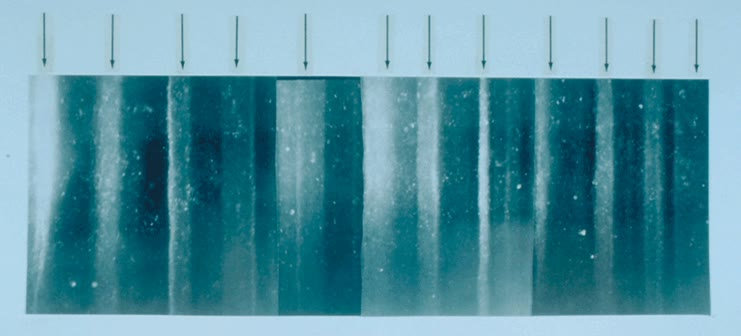
\includegraphics[width=0.72\linewidth]{images/book4/b2-24-gisp2-layers.jpg}
\par\smallskip{\small مقطع من العيّنة الجليدية GISP2 من وسط غرينلاند من عمق \qty{1855}{m}،
مُضاء من الأسفل، تتناوب فيه طبقات الصيف والشتاء (الأسهم أسهم
الشريحة الأصلية). ففي أثناء الصيف الشمالي الجافّ، تحمل الريح الغبار من القطب الشمالي الكندي وساحل غرينلاند
إلى الغطاء الجليدي.
الصورة: \mbox{\textdir TLT Anthony Gow}، مختبر CRREL التابع لسلاح المهندسين في الجيش الأمريكي، مجموعة شرائح المناخ القديم للإدارة الوطنية للمحيطات والغلاف الجوي، ملك عام،
عبر \mbox{\textdir TLT Wikimedia Commons}.}
\end{omfigure}
% ledger: photo:b2-24-gisp2, noaa:gisp2-layers

\begin{inthelab}[تقطيع عيّنة جليدية]
\begin{minipage}[t]{0.54\linewidth}\vspace{0pt}
في مرفق وطني للعيّنات الجليدية، تُحفظ العيّنات في أنابيب، مترًا واحدًا من العيّنة لكلّ أنبوب، في
مُجمِّد أرشيفي عند \qty{-36}{\celsius}؛ ويعمل العلماء في غرفة فحص عند
\qty{-24}{\celsius}. وحين تصل عيّنة جديدة، يتشكّل خطّ لمعالجة العيّنة: فيقيس العلماء
والفنّيون كلّ مقطع ويفهرسونه ويقطعونه، بمعدّل نموذجي من 30 إلى \qty{35}{m} في اليوم، بحيث
تستغرق عيّنة طولها \qty{1000}{m} من ستّة إلى ثمانية أسابيع. ويسوّي أحد الباحثين سطح العيّنة
بمِسحاج ويقيس ناقليّتها الكهربائية، وهي مفتاح لتحديد الطبقات وتأريخها؛ ويقطع آخر
بالمنشار القطع التي سيُحلَّل هواؤها المحتبس بحثًا عن ثاني أكسيد الكربون والميثان؛ ثم تُشحن العيّنات
إلى المختبرات التي تقيسها. وفي موقع EPICA في القبّة C، كانت كلّ عيّنة من مقطع \mbox{\textdir TLT $\delta$D}
\qty{55}{cm} من الجليد.
\end{minipage}\hfill
\begin{minipage}[t]{0.42\linewidth}\vspace{0pt}
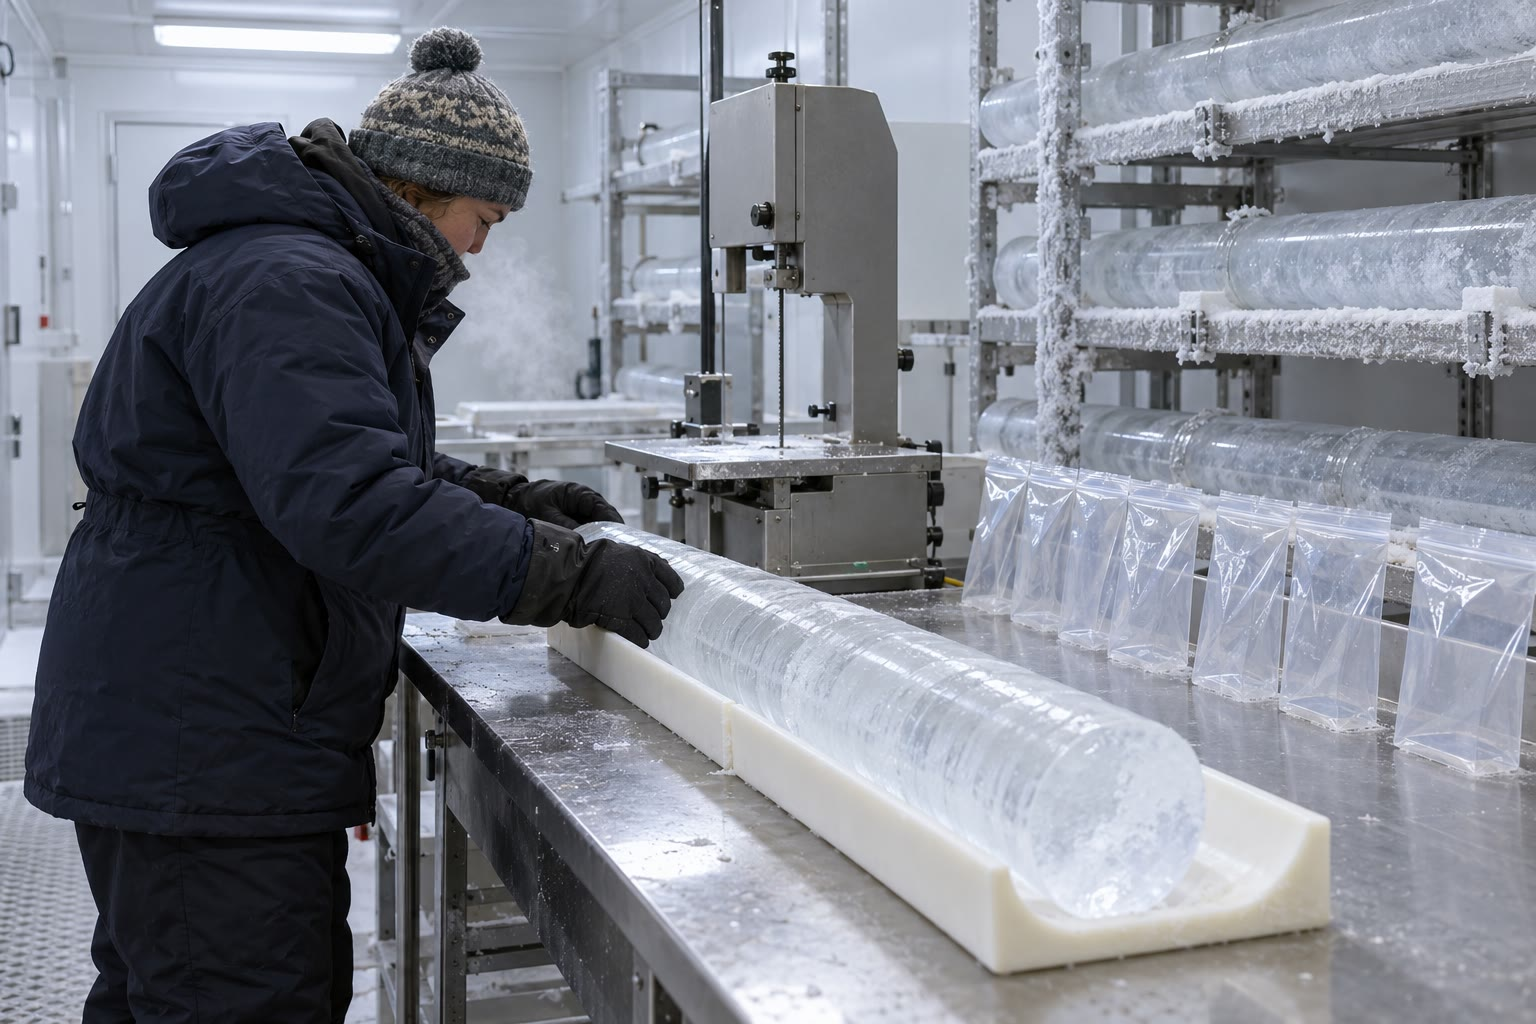
\includegraphics[width=\linewidth]{images/book4/ai/b2-24-cold-lab.jpg}

{\scriptsize قطعة من عيّنة جليدية على طاولة مختبر بارد، بجانب منشار شريطي وأكياس
عيّنات (رسم توضيحي مولَّد بالذكاء الاصطناعي).}
\end{minipage}
\end{inthelab}
% ledger: nsficf:cpl, jouzel07:edc-corr

\section{مؤشّرات بديلة أخرى، وأرشيفات أخرى}\label{sec:b2:climate-proxies:others}

\subsection*{مغنيسيوم الأصداف}

يأخذ كالسيت المنخربات قليلًا من المغنيسيوم مكان الكالسيوم، ويأخذ أكثر منه حين
يكون الماء أدفأ. ولا تتوقّف النسبة على التركيب النظائري للماء، فهي
تعطي درجة الحرارة التي تحتاج إليها معادلة \mbox{\textdir TLT $\delta^{18}$O}.

\begin{definition}[نسبة Mg/Ca (مؤشّرًا بديلًا)]\label{def:b2:climate-proxies:mgca}
\emph{نسبة Mg/Ca (مؤشّرًا بديلًا)}\index{نسبة Mg/Ca (مؤشّرًا بديلًا)} هي نسبة المغنيسيوم إلى الكالسيوم في
كالسيت أصداف المنخربات، بوحدة \unit{mmol/mol}، وتُستعمل مقياسًا لدرجة حرارة
الماء الذي نمت فيه الصدفة عبر معايرة أسّية
\[
  \text{Mg/Ca} = B\,\mathrm{e}^{A T},
\]
حيث $A$ قريب من \qty{0.09}{\per\celsius} للأنواع العوالق و$B$ خاصّ بالنوع.
\end{definition}
% ledger: groeneveld19:anand, morley24:mgca, miller20:paleotemp

مع $A = 0.09$ تنمو النسبة بمقدار $\mathrm{e}^{0.09} - 1 = \qty{9.4}{\percent}$ لكلّ درجة،
أيًّا كانت درجة الحرارة. ولنوع عالق من المياه الباردة، المعايرة المتوقَّعة من
درجة الحرارة وحدها هي $\text{Mg/Ca} = 0.4\,\mathrm{e}^{0.09T}$؛ وتوفيق على 235 صدفة من شباك
العوالق ومن قمم عيّنات شمال الأطلسي يعطي $0.372\,\mathrm{e}^{0.0936T}$، مع $r^2 = 0.90$.
وعند درجات الحرارة المنخفضة تحيد النسب المقيسة عن المنحنى، ويُعزى الحيود إلى
تركيز أيون الكربونات في ماء البحر: \omterm{def:b2:climate-proxies:proxy}{فالمؤشّر البديل} نادرًا ما يتوقّف على متغيّر واحد فقط.
والأنواع القاعية أقلّ حساسية، بنحو \qty{0.1}{mmol/mol} لكلّ درجة للأنواع الفقيرة بالمغنيسيوم
التي تعيش داخل الرسوبيات.
% ledger: morley24:mgca, wharton26:deep

\begin{omfigure}
\centering
% figdata/bachelor-2/proxies.py part calib
\begin{tikzpicture}
\begin{groupplot}[group style={group size=2 by 1, horizontal sep=1.7cm},
  tick label style={font=\scriptsize}, label style={font=\small}, height=5.2cm,
  width=0.48\linewidth]
\nextgroupplot[xmin=-2, xmax=14, ymin=0, ymax=3.8, xlabel={درجة الحرارة $T$ \babelsublr{(\unit{\celsius})}},
  ylabel={الفرق $\delta^{18}\mathrm{O}_{\mathrm{b}} - \delta^{18}\mathrm{O}_{\mathrm{sw}}$ \babelsublr{(\unit{\permil})}},
  xtick={0,4,...,12}, title={\foreignlanguage{arabic}{أ\enspace قيمة \mbox{\textdir TLT $\delta^{18}$O} القاعية}}, title style={font=\scriptsize}]
\addplot[black, thick] table[x=T, y=dd_benthic] {figdata/out/bachelor-2-proxies-calib.dat};
\nextgroupplot[xmin=0, xmax=30, ymin=0, ymax=6.5, xlabel={درجة الحرارة $T$ \babelsublr{(\unit{\celsius})}},
  ylabel={\babelsublr{Mg/Ca (\unit{mmol/mol})}}, xtick={0,5,...,30}, title={\foreignlanguage{arabic}{ب\enspace نسبة Mg/Ca لدى العوالق}},
  title style={font=\scriptsize},
  legend style={font=\scriptsize, at={(0.03,0.97)}, anchor=north west, draw=none},
  legend cell align=left]
\addplot[ocRed, thick] table[x=T, y=mgca_pred] {figdata/out/bachelor-2-proxies-calib.dat};
\addlegendentry{$0.4\,\mathrm{e}^{0.09T}$}
\addplot[ocBlue, thick, densely dashed] table[x=T, y=mgca_fit]
  {figdata/out/bachelor-2-proxies-calib.dat};
\addlegendentry{$0.372\,\mathrm{e}^{0.0936T}$}
\end{groupplot}
\end{tikzpicture}
\par\smallskip{\small معايرتان. (أ) المعايرة القاعية في
\cref{prop:b2:climate-proxies:benthic}: الكالسيت أثقل من الماء (كلّ على
مقياسه) بمقدار \num{0.21} بالجزء في الألف إضافيةً لكلّ درجة تبرّد. (ب) نسبة Mg/Ca لنوع
عالق، كما تُتوقَّع من درجة الحرارة وحدها وكما وُفّقت على 235 صدفة.}
\end{omfigure}
% ledger: miller20:paleotemp, morley24:mgca

مقيستين على الأصداف نفسها، تعطي Mg/Ca و\mbox{\textdir TLT $\delta^{18}$O} معادلتين لمجهولين: فنسبة Mg/Ca
تعطي $T$، ثم تعطي \cref{prop:b2:climate-proxies:benthic}
$\delta^{18}\mathrm{O}_{\mathrm{sw}}$، أي إشارة حجم الجليد. وبتطبيقها على أصداف قاعية من
أعماق شمال غرب الأطلسي، تجد الطريقة أن ماء الذروة الجليدية الأخيرة كان أبرد من ماء اليوم
بنحو \qty{2}{\celsius} فقط ($-1.78 \pm \qty{0.56}{\celsius}$)، بينما تضع تقديرات
ماء المسام كتلتي الماء العميق كلتيهما قرب التجمّد في المحيط الجليدي، عند $-1.1$
و\qty{-1.9}{\celsius}، حيث تكونان اليوم عند 2 إلى \qty{4}{\celsius} و0 إلى \qty{1}{\celsius}.
% ledger: miller20:paleotemp, wharton26:deep

\subsection*{حلقات الأشجار}

\begin{definition}[علم المناخ الشجري؛ التأريخ المتقاطع]\label{def:b2:climate-proxies:dendro}
\emph{علم المناخ الشجري}\index{علم المناخ الشجري} هو إعادة بناء المناخ الماضي من
حلقات النموّ السنوية للأشجار: عرضها، وكثافة خشبها وتركيبها
النظائري. و\emph{التأريخ المتقاطع}\index{التأريخ المتقاطع} هو مطابقة نمط الحلقات العريضة
والضيّقة بين الأشجار، وهو ما يعيّن لكلّ حلقة سنتها التقويمية المطلقة ويكشف
الحلقات الغائبة محلّيًّا في شجرة واحدة.
\end{definition}
% ledger: bebchuk26:crossdating, bebchuk26:absent-rings, ncei:tree-ring, ncei:proxy

تكون الحلقة أعرض حين تلائم الظروف النموّ. \omterm{def:b2:climate-proxies:dendro}{والتأريخ المتقاطع} موثوق في المواقع ذات المناخ المتطرّف، حيث يحدّ
عامل مناخي واحد نموّ الأشجار كلّها، فتشترك في النمط نفسه؛ وقد
يفشل حيث لا يهيمن عامل واحد، وحيث تغيب حلقات كثيرة محلّيًّا.
وبتراكب أنماط الأشجار الحيّة والأخشاب القديمة والخشب المدفون يمتدّ التسلسل الزمني إلى الوراء
سنة بسنة؛ فقد أرّخت دراسة حديثة تسلسلًا زمنيًّا من 100 شجرة طقسوس شبه أحفورية من شرق إنجلترا بفترة
456 سنة ممتدّة من 2668 إلى 2213 قبل الميلاد، مستعملة \mbox{\textdir TLT $\delta^{18}$O} في أكثر من \num{1500} من حلقاتها
مقابل تسلسل زمني للبلّوط مؤرَّخ تأريخًا مطلقًا. ويحفظ بنك البيانات الدولي لحلقات الأشجار عروض
الحلقات وكثافاتها ونظائرها وتسلسلاتها الزمنية لأكثر من \num{5000} موقع في ستّ قارّات.
% ledger: ncei:proxy, bebchuk26:crossdating, bebchuk26:absent-rings, ncei:tree-ring

\subsection*{الكهوف والبحيرات}

\begin{definition}[الرواسب الكهفية؛ الفارفة]\label{def:b2:climate-proxies:archives}
\emph{الرواسب الكهفية}\index{الرواسب الكهفية} رواسب معدنية تتكوّن من المياه الجوفية داخل
الكهف: الصواعد والهوابط وأشكال أخرى. و\emph{الفارفة}\index{الفارفة} هي
راسب سنة واحدة في رسوبيات قاع بحيرة أو بحر، وهي عادةً زوج من الصفائح متباينة
التركيب، تترسّب إحداهما في الصيف والأخرى في بقيّة السنة.
\end{definition}
% ledger: ncei:speleothem, mccarthy23:varves

تنمو \omterm{def:b2:climate-proxies:archives}{الرواسب الكهفية} طبقة فوق طبقة من المياه الجوفية التي تبلغ الكهف؛ وسماكة
طبقاتها وسجلّاتها النظائرية تعطي ظروف المناخ الماضي. وبعضها ذو أشرطة سنوية،
وبعضها يحتوي على مركّبات يمكن تأريخها إشعاعيًّا. ويتّفق السلّم الزمني لعيّنات غرينلاند مع سلّم
\omterm{def:b2:climate-proxies:archives}{الرواسب الكهفية} في كهف هولو بفارق لا يتجاوز 800 سنة على مدى آخر \num{60000} سنة: أرشيفان،
أُرّخا بطريقتين مختلفتين، يتحقّق كلّ منهما من الآخر.
% ledger: ncei:speleothem, svensson08:gicc05

\begin{omfigure}
\centering
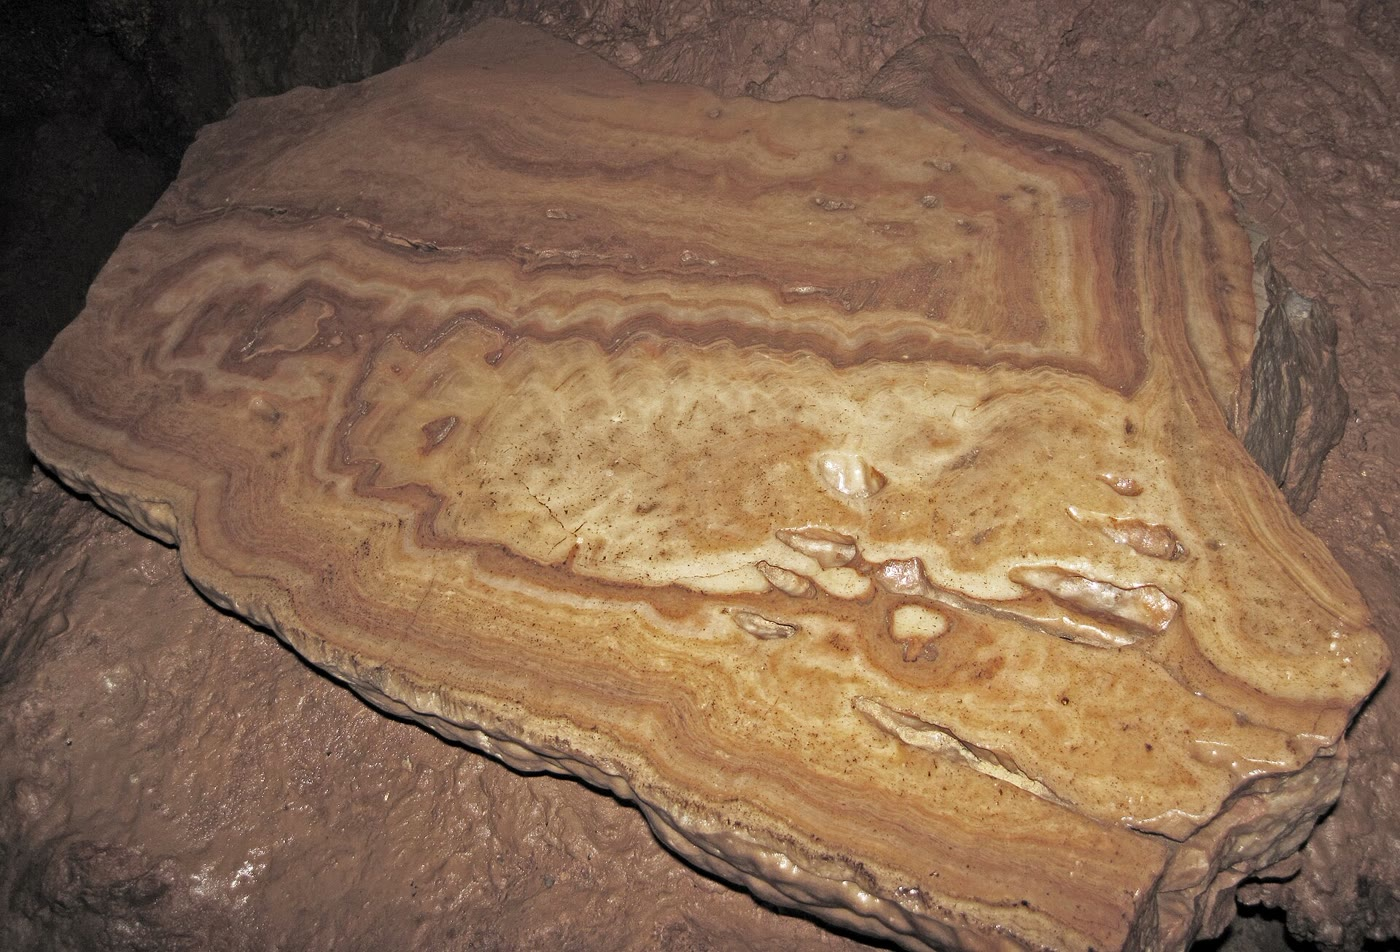
\includegraphics[width=0.62\linewidth]{images/book4/b2-24-speleothem.jpg}
\par\smallskip{\small مقطع مقطوع ومصقول من رواسب كهفية كالسيتية من كهوف دايموند في
كنتاكي، ملوّن بشوائب أكسيد الحديد: كلّ شريط كان يومًا سطح الراسب.
الصورة: \mbox{\textdir TLT James St.~John, CC~BY~2.0 (Wikimedia Commons)}.}
\end{omfigure}
% ledger: photo:b2-24-speleothem

في الحوض العميق لبحيرة كروفورد، في أونتاريو، لا يؤوي الماء القاعي، الأملح والأكثر قلوية من
الماء الذي فوقه، حيوانات كبيرة بما يكفي لتحريك الطين، مع أنه جيّد
الأكسجة، وكلّ سنة تضيف زوجًا من الطبقات: طبقة من المادة العضوية، يعلوها
الكالسيت الذي يترسّب كلّ صيف من الماء السطحي القلوي. ورسوبيات البحيرات تحفظ أيضًا
حبوب لقاح الغطاء النباتي المحيط، التي تُقرأ بتحليل حبوب اللقاح؛ وسواء أكانت ذات فارفات أم لا، فهي تسجّل
اليابسة.
% ledger: mccarthy23:varves, mccarthy23:no-bioturbation, ncei:pollen

\section{نماذج العمر}\label{sec:b2:climate-proxies:age}

\omterm{def:b2:climate-proxies:proxy}{المؤشّر البديل} بلا تاريخ مجرّد طرفة. فكلّ أرشيف يحتاج إلى علاقة بين العمق، أو الحلقة، أو
الشريط، والعمر.

\begin{definition}[نموذج العمر؛ عدّ الطبقات السنوية]\label{def:b2:climate-proxies:age-model}
\emph{نموذج العمر}\index{نموذج العمر} هو الدالّة التي تعيّن عمرًا، مع شكّه، لكلّ
عمق من أعماق الأرشيف. و\emph{عدّ الطبقات السنوية}\index{عدّ الطبقات السنوية} يبني نموذج
عمر بعدّ الطبقات، من الأعلى إلى الأسفل، التي تسجّل كلّ منها سنة واحدة (طبقات الجليد، والفارفات،
والأشرطة)، وكلّ طبقة مشكوك في طابعها السنوي تُعدّ نصف سنة زائدًا أو ناقصًا
نصف سنة.
\end{definition}
% ledger: svensson08:gicc05, mccarthy23:varves

\begin{method}[بناء نموذج عمر]\label{met:b2:climate-proxies:age-model}
\begin{enumerate}
  \item حيث يكون للأرشيف طبقات سنوية، عُدَّها ابتداءً من قمّة معروفة، مسجّلًا الطبقات المشكوك فيها
        على حدة.
  \item حيث لا تكون له طبقات، أو يتعذّر تمييزها، ثبّت \emph{نقاط ربط}: أعماقًا مؤرَّخة
        تأريخًا مستقلًّا، بالكربون المشعّ أو بطرائق إشعاعية أخرى، أو برماد بركاني مؤرَّخ، أو
        بمطابقة سجلّ جيّد التأريخ.
  \item بين نقاط الربط، استكمل خطّيًّا بالنسبة إلى العمق إذا لم يُعرف ما هو أفضل، أو بنموذج
        لكيفية تراكم الأرشيف وترقّقه.
  \item انقل شكّ كلّ خطوة إلى كلّ عمق.
\end{enumerate}
\end{method}
% ledger: svensson08:gicc05, noaa:gisp2-layers, ncei:speleothem

يعدّ التسلسل الزمني لعيّنات غرينلاند الجليدية 2005، GICC05، الطبقات السنوية في ثلاث عيّنات من غرينلاند،
وفي الجزء الجليدي في عيّنة NorthGRIP وحدها، على مدى آخر \num{60000} سنة؛ وتُعطى أعماره
بالسنوات قبل عام 2000 للميلاد، وتُكتب b2k. والطبقات المشكوك فيها، المعدودة $\frac12 \pm \frac12$،
تُجمع في \emph{الخطأ الأقصى للعدّ}، الذي يعدّه المؤلّفون انحرافين معياريين.
وعند بداية الهولوسين، 11\,703 سنة b2k، يبلغ 50 سنة؛ وعند بداية
الفترة البينية الدافئة 17 في غرينلاند، \num{59440} سنة b2k، يبلغ \num{1287} سنة.
% ledger: svensson08:gicc05, svensson08:table1

\begin{proposition}[نموّ خطأ العدّ]\label{prop:b2:climate-proxies:counting}
ليتضمّن عدٌّ $n$ طبقة مشكوكًا فيها، تُعدّ كلّ منها $\frac12$ بخطأ انحرافه
المعياري $\frac12$. فإذا كانت أخطاء الطبقات مستقلّة، كان الانحراف المعياري
للمجموع $\frac12\sqrt{n}$؛ وإذا كانت كلّها من الإشارة نفسها، كان خطأ المجموع
$\frac12 n$.
\end{proposition}

\begin{proof}
تباين مجموع أخطاء مستقلّة هو مجموع تبايناتها: $n \times
(\frac12)^2$، وجذره التربيعي $\frac12\sqrt{n}$. وإذا أخطأت كلّ طبقة في الاتجاه نفسه، فإن
الأخطاء تُجمع جمع الأعداد: $n \times \frac12$.
\end{proof}

عند GI-17، تعني السنوات \num{1287} من الخطأ الأقصى للعدّ \num{2574} طبقة مشكوكًا فيها. ولو كانت
أخطاؤها مستقلّة، لكان شكّ المجموع $\frac12\sqrt{2574} = 25$ سنة فقط.
والجمع الخطّي هو الخيار الحذر: فالطبقات المشكوك فيها في امتداد واحد من الجليد يحكم عليها
العادّون أنفسهم بالمعايير نفسها، ولا سبب لتوقّع أن تلغي أخطاؤها بعضها بعضًا.
وقد عدّ اثنان من المؤلّفين الجزء الأقدم من السجلّ كلّ على حدة؛ ويختلف عدّاهما
بأقلّ من الخطأ المطلق، وإن زاد الفرق محلّيًّا على خطأ العدّ النهائي. ويبلغ
متوسط الخطأ الأقصى للعدّ نحو \qty{1}{\percent} من الزمن الذي يغطّيه مقطع في الهولوسين
و\qty{5}{\percent} في الجزء الجليدي.
% ledger: svensson08:gicc05, svensson08:table1, svensson08:two-counters

\begin{omfigure}
\centering
% figdata/bachelor-2/proxies.py part gicc05
\begin{tikzpicture}
\begin{groupplot}[group style={group size=2 by 1, horizontal sep=1.7cm},
  tick label style={font=\scriptsize}, label style={font=\small}, height=5.4cm,
  width=0.48\linewidth, xmin=0, xmax=62, xlabel={العمر وفق \babelsublr{GICC05 (\unit{ka} b2k)}}]
\nextgroupplot[ymin=1450, ymax=2450, y dir=reverse, ylabel={العمق في \babelsublr{NorthGRIP (\unit{m})}},
  title={أ\enspace العمق والعمر}, title style={font=\scriptsize}]
\addplot[black, mark=*, mark size=1.1pt] table[x=age_ka, y=depth_m]
  {figdata/out/bachelor-2-proxies-gicc05.dat};
\nextgroupplot[ymode=log, ymin=2, ymax=30000, ylabel={الشكّ بالسنوات},
  title={ب\enspace شكّ العدّ}, title style={font=\scriptsize},
  legend style={font=\scriptsize, at={(0.03,0.97)}, anchor=north west, draw=none},
  legend cell align=left]
\addplot[ocRed, mark=*, mark size=1.1pt] table[x=age_ka, y=err_yr]
  {figdata/out/bachelor-2-proxies-gicc05.dat};
\addlegendentry{الخطأ الأقصى للعدّ}
\addplot[ocBlue, mark=o, mark size=1.1pt] table[x=age_ka, y=err_random_yr]
  {figdata/out/bachelor-2-proxies-gicc05.dat};
\addlegendentry{لو كانت مستقلّة}
\end{groupplot}
\end{tikzpicture}
\par\smallskip{\small التسلسل الزمني GICC05 عند 18 حدثًا مناخيًّا من بداية الهولوسين إلى
\qty{59.44}{ka}: (أ) العمق في عيّنة NorthGRIP مقابل العمر؛ ويتسطّح المنحنى كلّما ترقّقت الطبقات
السنوية مع العمق، فتشغل كلّ ألف سنة أمتارًا أقلّ من الجليد؛ (ب) الخطأ الأقصى للعدّ، والخطأ الذي يعطيه العدد نفسه من الطبقات
المشكوك فيها لو كانت أخطاؤها مستقلّة (\cref{prop:b2:climate-proxies:counting})؛
بمقياس لوغاريتمي. المعطيات: سفنسون وآخرون (2008)، الجدول 1.}
\end{omfigure}
% ledger: svensson08:table1, svensson08:gicc05

تترقّق الطبقات السنوية مع العمق، لأن الجليد يجري وينتشر وهو يغوص: فبين بداية
الهولوسين وGI-1، يبلغ متوسط سمك الطبقة \qty{3.75}{cm} في NorthGRIP؛ وبين GI-16
وGI-17، \qty{1.54}{cm}؛ وحول \qty{100}{ka}، تضعه نماذج الجريان قرب \qty{1}{cm}. وكلّما رقّت الطبقات، صعب
التمييز بينها.
% ledger: svensson08:table1, svensson08:gicc05

\section{المعايرة}\label{sec:b2:climate-proxies:calibration}

كلّ رقم يُقرأ من مؤشّر بديل يمرّ عبر معايرة.

\begin{definition}[معايرة المؤشّر البديل]\label{def:b2:climate-proxies:calibration}
\emph{معايرة المؤشّر البديل}\index{معايرة المؤشّر البديل} هي العلاقة التجريبية أو النظرية التي
تحوّل قيمة \omterm{def:b2:climate-proxies:proxy}{المؤشّر البديل} إلى المتغيّر المناخي الذي يقوم مقامه، وتُوضع على عيّنات
يُعرف فيها كلاهما، مع شكّها ومجال الظروف التي تكون فيها
صالحة.
\end{definition}
% ledger: morley24:mgca, miller20:paleotemp

العيّنات التي يُعرف فيها كلاهما حديثة: أصداف تُجمع بشباك العوالق، وقمم العيّنات اللبّية الرسوبية مقارنةً بالماء الذي فوقها، والثلج الحديث مقارنةً بدرجة
حرارة موقعه، والحلقات الخارجية للأشجار مقارنةً بسجلّات محطّة أرصاد.
ثم تُوفَّق العلاقة بالمربّعات الصغرى؛ ولقانون أسّي مثل معايرة Mg/Ca
يُجرى التوفيق على اللوغاريتم، الذي يحوّل $\text{Mg/Ca} = B\,\mathrm{e}^{AT}$ إلى
المستقيم $\ln(\text{Mg/Ca}) = \ln B + AT$. وتُتحقّق صحّة المعايرة على عيّنات
لم تُستعمل في توفيقها: فيُنحّى جزء من المعطيات الحديثة ويُتنبّأ به.
% ledger: morley24:mgca, werner18:slopes, ncei:tree-ring

تبقى ثلاثة حدود. فالمعايرة المقيسة عبر المكان، من مكان إلى آخر اليوم، قد لا تصحّ
عبر الزمن، كما بيّن جليد غرينلاند. والمعايرة المقيسة على مجال ظروف اليوم
يجب أن تُستقرأ بحذر: فنسبة Mg/Ca في الأصداف تحيد عن قانونها عند درجات الحرارة المنخفضة، حيث
يتولّى متغيّر آخر، هو أيون الكربونات، الأمر. والعلاقة الخطّية على مجال صغير
قد لا تكون خطّية على مجال كبير، كما هي حال \omterm{def:b2:climate-proxies:ice-volume}{أثر حجم الجليد}. وطريقة هذا الفصل
تجيب عنها بالطريقة نفسها: قِس مؤشّرين بديلين مستقلّين على العيّنة نفسها، ودع كلًّا منهما
يتحقّق من الآخر.
% ledger: werner18:slopes, morley24:mgca, rohling21:linear

\section*{التمارين}\label{sec:b2:climate-proxies:exercises}

معطيات التمارين، ما لم يُذكر غير ذلك: متوسط عمق المحيط $H = \qty{3682.2}{m}$، ومساحة
المحيط \qty{361.84e6}{km^2}؛ والمعايرة القاعية في \cref{prop:b2:climate-proxies:benthic}؛
والمعايرة للعوالق $\text{Mg/Ca} = 0.4\,\mathrm{e}^{0.09T}$ (\unit{mmol/mol}، \unit{\celsius})؛
وقيم $\delta$ للمياه والجليد بالجزء في الألف على مقياس \omterm{def:b2:isotope-geochemistry:standards}{VSMOW}، وللكالسيت بالجزء في الألف على مقياس \omterm{def:b2:isotope-geochemistry:standards}{VPDB}.
% ledger: charette:ocean-volume, miller20:paleotemp, morley24:mgca

\begin{exercise}[$\star$]\label{exo:b2:climate-proxies:1}
يحمل الجليد القارّي اليوم نحو \qty{27.5e6}{km^3} ويحمل المحيط \qty{1350e6}{km^3} من
الماء (خذ الحجوم كمّيات ماء). (أ) إذا كان متوسط \mbox{\textdir TLT $\delta^{18}$O} في الجليد $-30$ بالجزء في
الألف وفي المحيط 0، فما قيمة \mbox{\textdir TLT $\delta^{18}$O} في الغلاف المائي كلّه، بإهمال المياه
العذبة؟ (ب) لو ذاب الجليد كلّه، فماذا تصبح قيمة \mbox{\textdir TLT $\delta^{18}$O} في المحيط؟ (ج) ما
الكسر الذي يمثّله الجليد من الماء؟
\end{exercise}
% ledger: white13c9:ice-mass

\begin{exercise}[$\star$]\label{exo:b2:climate-proxies:2}
لصدفة قاعية القيمة $\delta^{18}\mathrm{O}_{\mathrm{b}} = 2.50$ بالجزء في الألف. (أ) احسب
درجة حرارتها لو كان لماء البحر $\delta^{18}\mathrm{O}_{\mathrm{sw}} = 0$. (ب) احسبها لو كان
لماء البحر $+1.0$ بالجزء في الألف. (ج) لصدفة أخرى، من الماء نفسه عند $0$ بالجزء في الألف، القيمة
$2.71$ بالجزء في الألف: بكم كان ماؤها أبرد؟
\end{exercise}
% ledger: miller20:paleotemp

\begin{exercise}[$\star$]\label{exo:b2:climate-proxies:3}
(أ) احسب نسبة Mg/Ca في معايرة العوالق عند \qty{10}{\celsius} وعند
\qty{20}{\celsius}. (ب) بأيّ عامل تنمو النسبة على هذه الدرجات العشر، وبأيّ
نسبة مئوية لكلّ درجة؟ (ج) احسب درجة حرارة أصداف نسبتها Mg/Ca = 2.0
و\qty{1.0}{mmol/mol}.
\end{exercise}
% ledger: morley24:mgca

\begin{exercise}[$\star$]\label{exo:b2:climate-proxies:4}
يمتدّ تسلسل زمني لأشجار طقسوس شبه أحفورية من 2668 إلى 2213 قبل الميلاد. (أ) كم سنة يغطّي،
بعدّ سنتي الطرفين كلتيهما؟ (ب) لماذا يستحقّ التسلسل الزمني المبنيّ من أشجار كثيرة ثقة أكبر من
عدّ حلقات شجرة واحدة؟ (ج) لماذا تتوقّع أن يكون \omterm{def:b2:climate-proxies:dendro}{التأريخ المتقاطع} أسهل لأشجار
قرب خطّ الأشجار البارد منه لأشجار غابة منخفضة معتدلة رطبة؟
\end{exercise}
% ledger: bebchuk26:crossdating

\begin{exercise}[$\star\star$]\label{exo:b2:climate-proxies:5}
(أ) باستعمال \cref{prop:b2:climate-proxies:mass-balance}، احسب \omterm{def:b2:climate-proxies:ice-volume}{أثر حجم الجليد} لانخفاض في مستوى البحر
قدره \qty{125}{m} وقدره \qty{134}{m}، مع جليد عند $-40$ بالجزء في الألف. (ب) احسبه لانخفاض
\qty{130}{m} مع جليد عند $-30$ و$-35$ و$-50$ بالجزء في الألف. (ج) أيّ متوسط تركيب للجليد
يجعل أثر انخفاض قدره \qty{130}{m} مساويًا للقيمة \num{1.0} بالجزء في الألف المقيسة في مياه
المسام؟ قارن بتراكيب الأغطية الجليدية الحالية.
\end{exercise}
% ledger: ipcc:lgm-sea, white:d18o, miller20:ice-cal, wharton26:deep

\begin{exercise}[$\star\star$]\label{exo:b2:climate-proxies:6}
قارن بين المعايرتين لنسبة Mg/Ca في النوع العالق نفسه: المتوقَّعة من
درجة الحرارة وحدها، $0.4\,\mathrm{e}^{0.09T}$، والموفَّقة $0.372\,\mathrm{e}^{0.0936T}$. (أ) عند
أيّ درجة حرارة تتّفقان؟ (ب) عند \qty{2}{\celsius}، بأيّ نسبة مئوية تكون النسبة الموفَّقة
أدنى من المتوقَّعة؟ (ج) صدفة نمت عند \qty{2}{\celsius} تتبع القانون الموفَّق؛ فأيّ
درجة حرارة يعطيها لها القانون المتوقَّع؟
\end{exercise}
% ledger: morley24:mgca

\begin{exercise}[$\star\star$]\label{exo:b2:climate-proxies:7}
في عيّنة NorthGRIP، تقع بداية الهولوسين عند \qty{1492.45}{m} و\num{11703} سنة
b2k، وبداية GI-1 عند \qty{1604.64}{m} و\num{14692} سنة؛ وبداية GI-16 عند
\qty{2402.55}{m} و\num{58280} سنة، وبداية GI-17 عند \qty{2420.44}{m} و\num{59440} سنة.
(أ) احسب متوسط سمك الطبقات السنوية في كلّ فترة. (ب) لماذا تكون أرقّ
في الأعماق الأكبر؟ (ج) لماذا يصبح \omterm{def:b2:climate-proxies:age-model}{عدّ الطبقات السنوية} مستحيلًا عند عمق ما؟
\end{exercise}
% ledger: svensson08:table1, svensson08:gicc05

\begin{exercise}[$\star\star$]\label{exo:b2:climate-proxies:8}
استعمل أوّل نقطتي ربط في \cref{exo:b2:climate-proxies:7}، مع خطأين أقصيين للعدّ قدرهما 50
و93 سنة. (أ) بالاستكمال الخطّي بالنسبة إلى العمق، أعطِ عمر الجليد عند \qty{1550}{m}.
(ب) عبّر عنه بالسنوات قبل 1950. (ج) استكمل الشكّ بالطريقة نفسها.
\end{exercise}
% ledger: svensson08:table1

\begin{exercise}[$\star\star$]\label{exo:b2:climate-proxies:9}
يبلغ الخطأ الأقصى للعدّ في GICC05 ما قدره 93 سنة عند GI-1 و\num{1287} سنة عند GI-17. (أ) كم
طبقة مشكوكًا فيها يمثّل كلّ منهما؟ (ب) ماذا يكون الشكّ لو كانت أخطاء هذه
الطبقات مستقلّة، انحراف كلّ منها المعياري نصف سنة؟ (ج) بأيّ عامل يتجاوز
الجمع الخطّي التقدير المستقلّ في كلّ حالة، ولماذا ينمو العامل مع العمق؟
\end{exercise}
% ledger: svensson08:gicc05, svensson08:table1

\begin{exercise}[$\star\star\star$]\label{exo:b2:climate-proxies:10}
في موقع EPICA في القبّة C يبلغ متوسط \mbox{\textdir TLT $\delta$D} في الجليد $-396.6$ بالجزء في الألف على مدى آخر ألفي سنة
و$-441.7$ بالجزء في الألف على مدى الفترة من 19 إلى \qty{23}{ka}. (أ) الميل المكاني لقيمة \mbox{\textdir TLT $\delta^{18}$O} في القارة القطبية الجنوبية
\num{0.8} بالجزء في الألف لكلّ درجة. حوّله، بخطّ الماء الجوّي، إلى ميل لقيمة \mbox{\textdir TLT $\delta$D}
وقدّر التبرّد الجليدي. (ب) كان المحيط الجليدي أثقل بمقدار \num{1.0} بالجزء في الألف في
\mbox{\textdir TLT $\delta^{18}$O}، فكان الثلج المتكوّن منه أثقل أيضًا. بافتراض أن \mbox{\textdir TLT $\delta$D} في المحيط
تغيّرت ثماني مرّات أكثر، صحّح \mbox{\textdir TLT $\delta$D} الجليدية وقدّر التبرّد من جديد.
(ج) الشذوذ المنشور $-0.09$ و\qty{-9.39}{\celsius} للفترتين؛ فأيّ ميل لقيمة
\mbox{\textdir TLT $\delta$D} لكلّ درجة يقتضيه ذلك، وأيّ تصحيح آخر تتضمّنه السلسلة المنشورة؟
\end{exercise}
% ledger: data:b4-proxies, werner18:slopes, kc98:mwl, wharton26:deep, jouzel07:edc-corr

\begin{exercise}[$\star\star\star$]\label{exo:b2:climate-proxies:11}
تستعمل معايرة لنسبة Mg/Ca في نوع عالق ستّ عيّنات من قمم العيّنات اللبّية (درجة حرارة الماء،
وMg/Ca بوحدة \unit{mmol/mol}): (4، 0.59)، (8، 0.80)، (12، 1.21)، (16، 1.65)، (20، 2.47)، (24، 3.41).
(أ) وفّق $\ln(\text{Mg/Ca}) = \ln B + AT$ بالمربّعات الصغرى، وأعطِ $A$ و$B$. (ب) احسب
بواقي اللوغاريتم، وقارن التوفيق بالقانون $0.4\,\mathrm{e}^{0.09T}$. (ج) أعطِ
درجة حرارة صدفة جليدية نسبتها Mg/Ca = 1.30. (د) لصدفة النسبة Mg/Ca = 0.45: احسب
درجة حرارتها، وبيّن لماذا تستحقّ هذه القيمة ثقة أقلّ من السابقة.
\end{exercise}
% ledger: morley24:mgca

\begin{exercise}[$\star\star\star$]\label{exo:b2:climate-proxies:12}
ينمو غطاء جليدي على مرحلتين: أوّلًا يُختزن \qty{60}{m} من مستوى البحر جليدًا عند $-30$ بالجزء في الألف،
ثم \qty{70}{m} أخرى جليدًا عند $-45$ بالجزء في الألف. (أ) بيّن أن موازنة الكتلة في
\cref{prop:b2:climate-proxies:mass-balance} تصبح $(H - h)\,\Delta\delta = -\sum_i h_i\delta_i$
لعدّة مخازن من الجليد، واحسب \omterm{def:b2:climate-proxies:ice-volume}{أثر حجم الجليد} بعد كلّ مرحلة. (ب) ما متوسط
تركيب الجليد في النهاية؟ (ج) قاعدة خطّية، معايَرة على الحالة النهائية، تحوّل
$\Delta\delta$ إلى مستوى بحر. فأيّ انخفاض في مستوى البحر تستنتجه للمرحلة الأولى، ولماذا
تخطئ؟
\end{exercise}
% ledger: rohling21:linear, white:d18o, miller20:ice-cal

\begin{problem}[{مسألة نهاية الأسبوع --- صدفة واحدة، وإشارتان}]\label{pb:b2:climate-proxies:1}
بكم كان المحيط العميق أبرد في الذروة الجليدية الأخيرة؟ إن \mbox{\textdir TLT $\delta^{18}$O} في الأصداف القاعية
يمزج الجواب بحجم الجليد؛ وهذه المسألة تفصل بينهما. استعمل معطيات
التمارين؛ فقد كان مستوى البحر أدنى من مستواه اليوم بمقدار 125 إلى \qty{134}{m}، ويُظنّ أن جليد الغطاء
الجليدي لأمريكا الشمالية كانت قيمة \mbox{\textdir TLT $\delta^{18}$O} فيه نحو $-40$ بالجزء في الألف.

\medskip\noindent\textbf{الجزء الأول --- الجليد على اليابسة.}
\begin{enumerate}
  \item احسب حجم الماء المنزوع من المحيط بانخفاض في مستوى البحر قدره \qty{130}{m}.
  \item احسب \omterm{def:b2:climate-proxies:ice-volume}{أثر حجم الجليد} لهذا الانخفاض مع جليد عند $-40$ بالجزء في الألف.
  \item احسبه لانخفاضين قدرهما \qty{125}{m} و\qty{134}{m}.
  \item احسبه لانخفاض \qty{130}{m} مع جليد عند $-35$ وعند $-50$ بالجزء في الألف. أيّ الشكّين
        أهمّ، شكّ مستوى البحر أم شكّ الجليد؟
  \item تعطي مياه مسام الرسوبيات الجليدية $1.0 \pm 0.1$ بالجزء في الألف. فأيّ متوسط تركيب
        للجليد يتطلّبه انخفاض قدره \qty{130}{m} لإنتاج ذلك؟
  \item احسب الانزياح لكلّ متر من مستوى البحر للانخفاضات الصغيرة مع جليد عند $-40$ بالجزء في الألف،
        وقارنه بالقيمة \num{0.011} بالجزء في الألف لكلّ متر المستمدّة من مستويات البحر المؤرَّخة.
\end{enumerate}

\medskip\noindent\textbf{الجزء الثاني --- ميزانا حرارة.}
\begin{enumerate}[resume]
  \item بيّن من \cref{prop:b2:climate-proxies:benthic} أن التبرّد بمقدار \qty{1}{\celsius} مع
        ثبات تركيب الماء يرفع $\delta^{18}\mathrm{O}_{\mathrm{b}}$ بمقدار \num{0.21} بالجزء في الألف.
  \item احسب $\delta^{18}\mathrm{O}_{\mathrm{b}}$ لصدفة قاعية نمت اليوم في ماء عند
        \qty{2.0}{\celsius} مع $\delta^{18}\mathrm{O}_{\mathrm{sw}} = 0$.
  \item احسبها لصدفة جليدية نمت في ماء عند \qty{-1.0}{\celsius} مع
        $\delta^{18}\mathrm{O}_{\mathrm{sw}} = +1.0$ بالجزء في الألف. ما التغيّر بين
        الصدفتين، وكم منه يعود إلى تركيب الماء؟
  \item لصدفة عالقة النسبة Mg/Ca = \qty{2.0}{mmol/mol}. احسب درجة حرارتها.
  \item تكسب الأصداف القاعية الفقيرة بالمغنيسيوم نحو \qty{0.1}{mmol/mol} لكلّ درجة. ولصدفة جليدية
        نسبة Mg/Ca أدنى بمقدار \qty{0.18}{mmol/mol} من صدفة حديثة من النوع نفسه ومن المكان
        نفسه. فأيّ تبرّد يدلّ عليه ذلك؟
  \item لماذا تعطي نسبة Mg/Ca درجة حرارة لا تتوقّف على حجم الجليد؟
\end{enumerate}

\medskip\noindent\textbf{الجزء الثالث --- الباقي.}
يقرأ المكدّس LR04 القيمة \num{3.23} بالجزء في الألف اليوم و\num{4.92} بالجزء في الألف في المتوسط على مدى الفترة من 19 إلى
\qty{23}{ka}.
\begin{enumerate}[resume]
  \item احسب تغيّر المكدّس بين اليوم والذروة الجليدية الأخيرة.
  \item لو كان كلّه أثرًا لحجم الجليد، مع جليد عند $-40$ بالجزء في الألف، فأيّ انخفاض في مستوى البحر
        يقتضيه (اعكس \cref{prop:b2:climate-proxies:mass-balance})؟ وهل يتّفق ذلك مع
        شواهد مستوى البحر؟
  \item خذ \omterm{def:b2:climate-proxies:ice-volume}{أثر حجم الجليد} في السؤال 2. ما الباقي لدرجة الحرارة،
        وأيّ تبرّد للماء العميق يعطيه؟
  \item خذ بدلًا من ذلك قيمة ماء المسام، \num{1.0} بالجزء في الألف. ما الباقي وما التبرّد؟
  \item تستعمل عملية إعادة بناء أخرى \num{0.25} بالجزء في الألف لكلّ درجة. أعد التقديرين بها.
  \item اليوم يكون ماء شمال الأطلسي العميق عند 2 إلى \qty{4}{\celsius} وماء القاع
        القطبي الجنوبي عند 0 إلى \qty{1}{\celsius}؛ وتضعهما مياه المسام عند $-1.1$ و\qty{-1.9}{\celsius}
        في المحيط الجليدي، وتجد نسبة Mg/Ca في الأصداف القاعية أن أعماق شمال غرب الأطلسي
        لم تكن أبرد إلا بنحو \qty{1.8}{\celsius}. فأيّ مجال من التبرّد تعطيه هذه، وأيّ
        التقديرين في السؤالين 15 و16 ترجّح؟
\end{enumerate}

\medskip\noindent\textbf{الجزء الرابع --- المنظر من الجليد.}
في موقع EPICA في القبّة C يبلغ متوسط \mbox{\textdir TLT $\delta$D} القيمة $-396.6$ بالجزء في الألف على مدى آخر ألفي سنة
و$-441.7$ بالجزء في الألف على مدى الفترة من 19 إلى \qty{23}{ka}؛ والشذوذ الحراري المنشور $-0.09$
و\qty{-9.39}{\celsius}.
\begin{enumerate}[resume]
  \item احسب تغيّر \mbox{\textdir TLT $\delta$D}.
  \item بميل لقيمة \mbox{\textdir TLT $\delta^{18}$O} قدره \num{0.8} بالجزء في الألف لكلّ درجة وبخطّ الماء الجوّي،
        قدّر التبرّد في القبّة C.
  \item احسب التبرّد المنشور، وميل \mbox{\textdir TLT $\delta$D} لكلّ درجة الذي يقتضيه.
  \item كان متوسط سطح الأرض العالمي أبرد بمقدار 5 إلى \qty{7}{\celsius} في الذروة الجليدية الأخيرة.
        رتّب تبرّدات القبّة C، والكرة الأرضية، والمحيط العميق.
  \item لماذا لا يمكن أن يكون المحيط العميق قد تبرّد بقدر ما تبرّد سطح القارة القطبية الجنوبية؟
  \item خلاصة القول: مع تصحيح حجم الجليد بقيمة ماء المسام، بكم كان المحيط العميق
        أبرد في الذروة الجليدية الأخيرة منه اليوم؟
\end{enumerate}
\end{problem}
% ledger: charette:ocean-volume, ipcc:lgm-sea, miller20:ice-cal, white:d18o, white13c9:ice-volume, wharton26:deep, miller20:paleotemp, morley24:mgca, data:b4-proxies, rohling21:linear, werner18:slopes, kc98:mwl, ipcc:lgm-cooling
